% This paper is prepared for the Review of Symbolic Logic (RSL).
% It uses the standard article class; converting to the Cambridge
% University Press (CUP) LaTeX class (jsl-rsl-cls) is mechanical
% and will be done at camera-ready stage.  RSL formatting conventions
% (theorem environments, bibliography style, MSC codes, keywords)
% are followed within the article class.
\documentclass[10pt, letterpaper]{article}

\usepackage[margin=1in]{geometry}
\usepackage[utf8]{inputenc}
\usepackage[T1]{fontenc}
\usepackage{lmodern}
\usepackage{amsmath, amssymb, amsthm}
\usepackage{booktabs}
\usepackage{graphicx}
\usepackage{xcolor}
\usepackage{hyperref}
\usepackage{enumitem}
\usepackage{caption, subcaption}
\usepackage{listings}
\usepackage{tikz}
\usetikzlibrary{positioning, fit, calc, arrows.meta, patterns}

% Theorem environments (RSL style: Theorem, Lemma, etc. numbered by section)
\newtheorem{theorem}{Theorem}[section]
\newtheorem{lemma}[theorem]{Lemma}
\newtheorem{proposition}[theorem]{Proposition}
\newtheorem{corollary}[theorem]{Corollary}
\theoremstyle{definition}
\newtheorem{definition}[theorem]{Definition}
\newtheorem{example}[theorem]{Example}
\theoremstyle{remark}
\newtheorem{remark}[theorem]{Remark}

% Lean code formatting
\lstdefinelanguage{Lean}{
  morekeywords={def, theorem, lemma, axiom, variable, inductive, structure,
    class, instance, where, match, with, by, exact, intro, apply, simp,
    rfl, fun, let, have, show, calc, if, then, else, do, return, sorry,
    namespace, end, open, import, section, Type, Prop, True, False,
    forall, exists, private, set, obtain, push_neg, unfold, constructor,
    rintro, refine, subst, rw, cases, induction, congr, ext},
  sensitive=true,
  morecomment=[l]{--},
  morecomment=[n]{/-}{-/},
  morestring=[b]",
  literate={→}{$\to$}1 {←}{$\leftarrow$}1 {↔}{$\leftrightarrow$}1
           {∀}{$\forall$}1 {∃}{$\exists$}1 {¬}{$\lnot$}1
           {∧}{$\land$}1 {∨}{$\lor$}1 {⟨}{$\langle$}1 {⟩}{$\rangle$}1
           {₁}{$_1$}1 {₂}{$_2$}1 {₀}{$_0$}1
           {⊊}{$\subsetneq$}1
           {≠}{$\neq$}1,
}
\lstset{
  language=Lean,
  basicstyle=\ttfamily\small,
  keywordstyle=\bfseries\color{blue!70!black},
  commentstyle=\itshape\color{green!50!black},
  stringstyle=\color{red!60!black},
  breaklines=true,
  columns=flexible,
  frame=single,
  framesep=4pt,
  xleftmargin=8pt,
  xrightmargin=8pt,
  aboveskip=8pt,
  belowskip=8pt,
}

% Notation
\newcommand{\Sach}{\mathsf{S}}
\newcommand{\World}{\mathsf{World}}
\newcommand{\Prop}{\mathsf{Prop}}
\newcommand{\eval}{\mathsf{eval}}
\newcommand{\expresses}{\mathsf{expresses}}
\newcommand{\structEq}{\sim_{\mathrm{struct}}}
\newcommand{\formEq}{\sim_{\mathrm{form}}}
\newcommand{\semEq}{\sim_{\mathrm{sem}}}
\newcommand{\Lean}{\textsc{Lean}}

\title{What \Lean{} Cannot Say:\\
A Machine-Checked Analysis of Wittgenstein's \emph{Tractatus}}
\author{Robb Walters}
\date{July 2026}

\begin{document}
\maketitle

\begin{abstract}
We present a machine-checked reconstruction of the semantic core
of \emph{Tractatus Logico-Philosophicus} in the \Lean{} proof
assistant.  The formalization models objects, states of affairs,
worlds, and propositions, and proves truth-functional
compositionality, functional completeness, and bivalence.

Beyond encoding, the system is parameterized over world models,
allowing a precise separation between (i)~structural invariants
of the propositional syntax, (ii)~model-dependent assumptions
such as the independence of atomic facts, and (iii)~formal limits
of expressibility.  We show that truth-functional compositionality
holds in all models, while independence characterizes a specific
``free'' model and fails in constrained models.

To analyze the relation between object language and metalanguage,
we introduce an \texttt{expresses} relation linking propositions
to meta-level predicates.  Using this, we prove that any
proposition expressing a world-independent property must be a
tautology or contradiction.  Consequently, nontrivial propositions
cannot express world-independent truths.

We further distinguish three notions of
equivalence---syntactic identity, logical-form equivalence up to
permutation, and semantic equivalence---and prove that the first
strictly refines the other two, which are themselves provably
incomparable: logical form neither determines nor is determined
by truth conditions.

We formalize Wittgenstein's $N$-operator (joint denial) and
settle TLP~5.52 in both directions: the quantifiers reduce to
$N$-applications over any finite domain, while over an infinite
domain no single $N$-application over finitely many instances
expresses the universal quantifier---the Geach--Soames critique
as a machine-checked theorem.  We also prove full functional
completeness (TLP~5.101): every truth-function on finitely many
atoms is realized by some proposition.

We give an exact characterization of the sayable---over finitely
many atoms, a world-property is expressible by a proposition iff
it is invariant under pointwise-$\iff$ agreement of worlds---and
show it fails over infinitely many atoms, where the totality
property of TLP~1 (``the world is everything that is the case'')
is invariant yet expressed by no proposition.

These results yield a formal decomposition of the \emph{Tractatus}
into invariants, assumptions, and limits, and provide a precise
characterization of the saying/showing distinction as a theorem
about expressibility in truth-functional languages.
The formalization comprises 2,148 lines of \Lean~4, proves 77
formally verified results with 0 \texttt{sorry} obligations
and 1 deliberate axiom (\texttt{axiom silence : True}, encoding
TLP~7).%
\footnote{The formalization is publicly available at
  \url{https://github.com/rjwalters/tractatus},
  with a browsable proof gallery at
  \url{https://leangenius.org/proof/tractatus-ontology}.
  It builds with \Lean~4 (toolchain \texttt{leanprover/lean4:v4.26.0}),
  depends on Mathlib (\texttt{import Mathlib.Tactic}), and compiles via
  \texttt{lake build}.  See Appendix~\ref{app:build} for full
  instructions.}
\end{abstract}

\medskip
\noindent
\textbf{Keywords:} Wittgenstein, \emph{Tractatus Logico-Philosophicus},
proof assistant, Lean~4, formal verification, truth-functional
semantics, saying/showing distinction, expressibility,
$N$-operator

\medskip
\noindent
\textbf{2020 Mathematics Subject Classification:}
03B70 (Logic in computer science),
03A05 (Philosophical and critical aspects of logic and foundations),
03B35 (Mechanization of proofs and logical operations)

% ================================================================
\section{Introduction}
\label{sec:intro}
% ================================================================

Wittgenstein's \emph{Tractatus Logico-Philosophicus}~\cite{wittgenstein1921}
proposes that the world consists of atomic facts (Sachverhalte),
that propositions are truth-functions of elementary propositions,
and that the limits of language are the limits of the world.
The text is terse, aphoristic, and deliberately resistant to
formalization---yet its semantic core is a precise theory of
truth-functional composition that invites formal reconstruction.

Several authors have pursued this invitation.
Lokhorst~\cite{lokhorst1988} provides a set-theoretic
reconstruction covering ontology, semantics, and propositional
attitudes;
Fogelin~\cite{fogelin1987} initiates the debate over expressive
completeness that Geach~\cite{geach1981} and
Soames~\cite{soames1983} develop;
Miller~\cite{miller1995} develops a Tractarian semantics for
predicate logic, responding in part to Fogelin and
Carruthers~\cite{carruthers1989};
Weiss~\cite{weiss2017} reconstructs the logical system with
$\Pi^1_1$-completeness results;
Stokhof~\cite{stokhof2008} traces the \emph{Tractatus}'s
influence on formal semantics.
These reconstructions clarify the \emph{Tractatus} as a semantic
system but are carried out on paper, without machine verification.
Separately, the proof-assistant community has formalized
philosophical arguments~\cite{benzmuller2017,fitelson2007} and
even complete metaphysical systems~\cite{scherf2025}, but a
Tractarian formalization has not appeared.

This paper contributes a machine-checked reconstruction in
\Lean~4~\cite{moura2021} that goes beyond encoding to yield new
analytical results.  Our central claim is:

\begin{quote}
\emph{The saying/showing distinction of the \emph{Tractatus} can
be reformulated as a theorem: nontrivial propositions cannot
express world-independent truths.}
\end{quote}

\noindent
This is not a paraphrase of Wittgenstein but a provable
consequence of the typed structure of the formalization.
The key device is an \texttt{expresses} relation (Definition~\ref{def:expresses})
that bridges the object language (propositions of type
$\mathsf{Proposition}\;\Sach$) and the metalanguage (terms of
type $\Prop$), making the object/meta boundary visible at the
type level.

More broadly, by parameterizing the formalization over a general
\texttt{WorldModel} structure, we show that the claims of the
\emph{Tractatus} decompose into three classes:
\begin{enumerate}[nosep]
  \item \textbf{Structural invariants} that hold in every world
    model---compositionality, bivalence, De Morgan duality.
  \item \textbf{Model-dependent assumptions} that hold in the
    unconstrained ``free'' model but fail in constrained
    models---principally, the independence of atomic facts.
  \item \textbf{Formal limits} on expressibility---the collapse
    of world-independent content to tautology or contradiction,
    and the strict separation of syntactic, logical-form, and
    semantic equivalence.
\end{enumerate}

\noindent
The specific contributions of this paper are:
\begin{enumerate}[nosep, label=(\arabic*)]
  \item A parameterized world-model abstraction that cleanly
    separates structural invariants from modeling assumptions,
    enabling precise identification of which Tractarian claims
    are theorems of the syntax and which are properties of a
    particular world model (Section~\ref{sec:formalization}).
  \item An \texttt{expresses} relation that makes the object/meta
    boundary a typed distinction, yielding the expressibility
    collapse theorem (Theorem~\ref{thm:collapse}): any proposition
    expressing a world-independent property is a tautology or
    contradiction (Section~\ref{sec:limits}).
  \item An equivalence analysis of three relations on
    propositions: syntactic identity strictly refines both
    logical-form equivalence and semantic equivalence, while the
    latter two are provably incomparable---logical form neither
    determines nor is determined by truth conditions.  The
    permutation-based $\formEq$ provides a formal candidate for
    Wittgenstein's ``logical form'' (Section~\ref{sec:hierarchy}).
  \item A formalization of the $N$-operator (joint denial)
    settling TLP~5.52 in both directions: proved for finite
    domains, and refuted---as a machine-checked theorem---for
    infinite ones, formalizing the Geach--Soames critique
    (Section~\ref{sec:noperator}).
  \item Full functional completeness (TLP~5.101): every
    truth-function on finitely many atoms is realized by some
    proposition, with the inhabitation hypothesis this genuinely
    requires (Section~\ref{sec:fullcompleteness}).
  \item An exact characterization of expressibility and the
    inexpressibility of totality: over finitely many atoms a
    world-property is expressible iff it is invariant under
    pointwise-$\iff$ agreement of worlds, whereas over infinitely
    many atoms the totality property of TLP~1 is invariant yet
    expressed by no proposition---a finite/infinite dichotomy
    turning on finite support (Section~\ref{sec:whatcanbesaid}).
  \item A three-way decomposition of all 77 formalized results
    into invariants, assumptions, and limits
    (Table~\ref{tab:decomposition}, Appendix~\ref{app:theorems}).
  \item A first-order extension using higher-order abstract syntax,
    proving compositionality lifts to quantified propositions
    (Section~\ref{sec:firstorder}).
\end{enumerate}

\noindent
The formalization comprises 2,148 lines of \Lean~4 across five
files.\footnote{%
  \texttt{TractatusOntology.lean} (1,345 lines, 45 theorem/lemma
  declarations), \texttt{TractatusQuantifiers.lean} (284 lines, 9),
  \texttt{TractatusNOperator.lean} (239 lines, 11),
  \texttt{TractatusCompleteness.lean} (142 lines, 9), and
  \texttt{TractatusExpressibility.lean} (138 lines, 3), plus 1
  deliberate axiom.  Appendix~\ref{app:theorems} lists every
  declaration.}
All proofs compile with 0 \texttt{sorry} obligations.
The sole axiom is \texttt{axiom silence : True} (TLP~7), a
deliberate boundary marker discussed in
Section~\ref{sec:limitations}.

The paper is organized as follows.
Section~\ref{sec:formalization} presents the formalization:
types, evaluation, and the world-model abstraction.
Section~\ref{sec:invariants} establishes the structural
invariants.
Section~\ref{sec:assumptions} analyzes the model-dependent
assumptions and exhibits countermodels.
Section~\ref{sec:limits} proves the expressibility results and
the separation of the three equivalence relations.
Section~\ref{sec:related} discusses related work.
Section~\ref{sec:discussion} reflects on the philosophical
implications and limitations.

% ================================================================
\section{The Formalization}
\label{sec:formalization}
% ================================================================

We formalize the ontological skeleton of the \emph{Tractatus}
in \Lean~4.  The design choices are deliberate modeling
decisions, not exegetical claims about Wittgenstein's intent.
We state them explicitly so that the reader can assess the
reconstruction's scope and limitations.

\begin{remark}[Choice of proof assistant]
\label{rem:lean4}
We use \Lean~4~\cite{moura2021} rather than Coq, Isabelle, or
Agda for three reasons: (i)~its dependent type theory allows
definitions and proofs to coexist naturally, which suits a
formalization that mixes data definitions with metatheorems;
(ii)~the Mathlib library provides automation
(\texttt{simp}, \texttt{tauto}, \texttt{push\_neg}) that keeps
proofs concise; and (iii)~\Lean's tactic mode allows readable
proof scripts that can be presented in a paper without excessive
notation overhead.
\end{remark}

\begin{remark}[Classical logic]
\label{rem:classical}
The formalization assumes classical logic throughout, via
\texttt{Classical.em} and related principles imported from
Mathlib.  This is a deliberate choice matching the
\emph{Tractatus}'s bivalent semantics: every proposition is
either true or false in every world (TLP~4.023).
Theorems depending essentially on classical reasoning include
bivalence, excluded middle as a tautology, double negation,
the expressibility collapse theorem, and contingent-proposition
variation.  A constructive formalization would require
restricting the world model or weakening several results.
\end{remark}

% ----------------------------------------------------------------
\subsection{Objects and States of Affairs}
\label{sec:objects}
% ----------------------------------------------------------------

TLP~2.02: ``The object is simple.''  Objects are the substance
of the world (TLP~2.021).  We model them as an abstract type
\texttt{TractObject} with no internal structure, capturing
Wittgenstein's insistence on simplicity.

A state of affairs (Sachverhalt) is a possible combination of
objects (TLP~2.01).  Rather than encoding the combinatorial
structure of objects into states of affairs, we index states of
affairs by an abstract type~$\Sach$:

\begin{lstlisting}
variable (TractObject : Type)
variable (Sachverhalt : Type)
\end{lstlisting}

\noindent
This choice leaves the internal structure of states of affairs
unspecified---an interpretive decision that captures independence
while remaining agnostic about combinatorial form (cf.\
TLP~2.0141).  We note explicitly that \texttt{TractObject} is
declared for conceptual completeness but plays no role in the
subsequent formal development, which begins at the level of
states of affairs; encoding the combination relation between
objects and Sachverhalte is future work
(Section~\ref{sec:limitations}).

% ----------------------------------------------------------------
\subsection{Worlds}
\label{sec:worlds}
% ----------------------------------------------------------------

TLP~1: ``The world is everything that is the case.''
A world is determined by which states of affairs obtain.  We
model this as a predicate:

\begin{lstlisting}
def World := Sachverhalt → Prop
\end{lstlisting}

\noindent
Every function $\Sach \to \Prop$ counts as a world.  This gives
the full Boolean cube of truth-value assignments, making the
independence of atomic facts (TLP~2.061) hold by construction.
We return to this modeling choice and its consequences in
Section~\ref{sec:assumptions}.

% ----------------------------------------------------------------
\subsection{Propositions}
\label{sec:propositions}
% ----------------------------------------------------------------

TLP~5: ``The proposition is a truth-function of elementary
propositions.''  We define propositions as an inductive type
built from elementary propositions, negation, and conjunction:

\begin{lstlisting}
inductive Proposition (S : Type) where
  | elementary : S → Proposition S
  | neg        : Proposition S → Proposition S
  | conj       : Proposition S → Proposition S → Proposition S
\end{lstlisting}

\noindent
Disjunction, implication, biconditional, and NAND are defined as
derived operations (TLP~5.101, 5.5), confirming that $\{\lnot, \land\}$
is an adequate basis.

% ----------------------------------------------------------------
\subsection{Semantic Evaluation}
\label{sec:eval}
% ----------------------------------------------------------------

The core semantic function interprets propositions against a
world:

\begin{lstlisting}
def Proposition.eval (p : Proposition S) (w : World S) : Prop :=
  match p with
  | .elementary s => w s
  | .neg q        => ¬ (q.eval w)
  | .conj q r     => q.eval w ∧ r.eval w
\end{lstlisting}

\noindent
An elementary proposition $\mathtt{elementary}\;s$ is true in
world~$w$ exactly when $w\;s$ holds.  Negation and conjunction
lift to their classical counterparts.%
\footnote{The formalization also provides a
\texttt{Bool}-valued evaluator \texttt{evalBool} for decidable
computation and proves its correctness against
\texttt{eval} (Theorem \texttt{evalBool\_correct}).
This engineering artifact enables \texttt{\#eval} demonstrations
but is not philosophically load-bearing.}

% ----------------------------------------------------------------
\subsection{Tautology, Contradiction, Nontriviality}
\label{sec:tautology}
% ----------------------------------------------------------------

A proposition is a \emph{tautology} if it holds in every world,
a \emph{contradiction} if it holds in none, and
\emph{nontrivial} if it holds in some world and fails in
another:

\begin{lstlisting}
def IsTautology (p : Proposition S) : Prop :=
  ∀ w : World S, p.eval w
def IsContradiction (p : Proposition S) : Prop :=
  ∀ w : World S, ¬ (p.eval w)
def Nontrivial (p : Proposition S) : Prop :=
  ∃ w₁ w₂ : World S, p.eval w₁ ∧ ¬ p.eval w₂
\end{lstlisting}

\noindent
We prove that nontriviality is equivalent to being neither a
tautology nor a contradiction.%
\footnote{Theorem \texttt{nontrivial\_iff\_not\_taut\_not\_contra}
  in \texttt{TractatusOntology.lean}.}

% ----------------------------------------------------------------
\subsection{General World Models}
\label{sec:worldmodel}
% ----------------------------------------------------------------

The definitions above hardwire the world model: every
function $\Sach \to \Prop$ is a world.  In many
applications---physics, epistemic logic, constrained
databases---not every assignment is legitimate.
We therefore introduce a \texttt{WorldModel} structure
that parameterizes the semantics:

\begin{lstlisting}
structure WorldModel (S : Type) where
  W        : Type
  holds    : W → S → Prop
  nonempty : Nonempty W
\end{lstlisting}

\noindent
The \emph{free model} \texttt{freeModel} recovers the original
semantics: $W = \Sach \to \Prop$ and \texttt{holds} is function
application.  We define a general evaluator \texttt{evalM} and
prove that \texttt{evalM (freeModel S)} agrees with
\texttt{Proposition.eval} (Theorem~\texttt{evalM\_free\_eq\_eval}).

This abstraction is the key structural device of the
formalization.  It allows us to state precisely which results
depend on the choice of world model and which do not.

% ================================================================
\section{Structural Invariants}
\label{sec:invariants}
% ================================================================

The following results hold in \emph{every} world model---they
are consequences of the inductive structure of propositions and
classical logic alone, with no assumptions about which worlds
exist.

% ----------------------------------------------------------------
\subsection{Truth-Functional Compositionality}
\label{sec:compositionality}
% ----------------------------------------------------------------

\begin{theorem}[Compositionality, model-independent]
\label{thm:compositionality}
For any world model $M$, any proposition $p$, and any two
worlds $w_1, w_2 \in M.W$: if $M.\mathit{holds}\;w_1\;s
\leftrightarrow M.\mathit{holds}\;w_2\;s$ for every state of
affairs~$s$, then $\eval_M\;p\;w_1 \leftrightarrow
\eval_M\;p\;w_2$.
\end{theorem}

\noindent
The proof is by structural induction on propositions.
The elementary case follows from the hypothesis; negation and
conjunction lift via \texttt{Iff.not} and \texttt{Iff.and}.

\begin{lstlisting}
theorem truth_functional_compositionality_gen (p : Proposition S)
    (w₁ w₂ : M.W)
    (h : ∀ s : S, M.holds w₁ s ↔ M.holds w₂ s) :
    evalM M p w₁ ↔ evalM M p w₂ := by
  induction p with
  | elementary s => exact h s
  | neg q ih     => simp only [evalM, ih]
  | conj q r ihq ihr => simp only [evalM, ihq, ihr]
\end{lstlisting}

\noindent
This establishes TLP~5 as a structural invariant: the
truth-value of a compound proposition is determined by its
elementary constituents regardless of which worlds the model
admits.

% ----------------------------------------------------------------
\subsection{Bivalence and Classical Tautologies}
\label{sec:bivalence}
% ----------------------------------------------------------------

Elementary bivalence (TLP~4.023) is an instance of classical
excluded middle:

\begin{theorem}[Bivalence]
For any state of affairs~$s$ and world~$w$: $w\;s \lor \lnot\;w\;s$.
\end{theorem}

\noindent
The standard tautologies follow: excluded middle ($p \lor
\lnot p$), double negation ($\lnot\lnot p \leftrightarrow p$),
De Morgan's laws, and modus ponens.  We verify each as a formal
theorem.  All of these results depend on \texttt{Classical.em}
(see Remark~\ref{rem:classical}).

% ----------------------------------------------------------------
\subsection{NAND Functional Completeness}
\label{sec:nand}
% ----------------------------------------------------------------

TLP~5.5 anticipates the Sheffer stroke.  We prove that negation
and conjunction are both expressible via NAND:

\begin{theorem}[NAND completeness]
\label{thm:nand}
For any propositions $p$, $q$ and world $w$:
\begin{enumerate}[nosep]
  \item $\mathtt{nand}(p, p).\eval\;w \leftrightarrow
    (\lnot p).\eval\;w$
  \item $(\lnot\;\mathtt{nand}(p, q)).\eval\;w \leftrightarrow
    (p \land q).\eval\;w$
\end{enumerate}
\end{theorem}

\noindent
Since $\{\lnot, \land\}$ generates all truth-functions and NAND
generates $\{\lnot, \land\}$, NAND alone is functionally
complete over the set of truth-functions expressible by the
proposition type---confirming TLP~5.5.

% ----------------------------------------------------------------
\subsection{Functional Completeness, Full Strength}
\label{sec:fullcompleteness}
% ----------------------------------------------------------------

The NAND result shows the interdefinability of the bases, but
TLP~5.101 claims more: \emph{every} truth-function of the
elementary propositions arises from the propositional basis.  We
prove this in full strength (\texttt{TractatusCompleteness.lean}):

\begin{theorem}[Functional completeness, TLP~5.101]
\label{thm:fc}
Let $\Sach$ be finite, decidable, and nonempty.  For every
truth-function $g : (\Sach \to \mathsf{Bool}) \to \mathsf{Bool}$
there is a proposition $p$ with
$p.\mathtt{evalBool}\;w = g\;w$ for every assignment~$w$.
\end{theorem}

\begin{lstlisting}
theorem functional_completeness {S : Type} [Fintype S] [DecidableEq S]
    [Nonempty S] (g : (S → Bool) → Bool) :
    ∃ p : Proposition S, ∀ w : S → Bool, p.evalBool w = g w
\end{lstlisting}

\noindent
The construction is the disjunctive normal form: for each
satisfying assignment $v$ of $g$, a \emph{minterm} conjoins, for
every atom $s$, the literal $\mathtt{elementary}\;s$ or its
negation according to $v\;s$; the minterms of all satisfying
assignments are then disjoined via the derived $\mathtt{disj}$.

\begin{remark}[\texttt{Nonempty S} is genuinely required]
\label{rem:fc-nonempty}
For empty $\Sach$ the type $\mathsf{Proposition}\;\Sach$ is
uninhabited (every proposition bottoms out in an elementary
leaf), while $(\Sach \to \mathsf{Bool}) \to \mathsf{Bool}$ still
has two elements---so nothing realizes the constant functions.
With at least one atom, the constants are realizable as
$p \lor \lnot p$ and $p \land \lnot p$.  Stating the theorem
surfaced this hypothesis: a small instance of the paper's
running theme that formalization forces modeling commitments
into the open.
\end{remark}

% ================================================================
\section{Model-Dependent Assumptions}
\label{sec:assumptions}
% ================================================================

Not every claim in the \emph{Tractatus} is a structural
invariant.  The independence of atomic facts---perhaps the most
famous ontological thesis of the text---is a property of a
specific world model.

% ----------------------------------------------------------------
\subsection{Independence in the Free Model}
\label{sec:independence}
% ----------------------------------------------------------------

We formalize independence as a typeclass:

\begin{lstlisting}
class IndependentWorlds (S : Type) where
  realizable : ∀ assignment : S → Prop,
    ∃ w : World S, ∀ s, w s ↔ assignment s
\end{lstlisting}

\noindent
The free model trivially satisfies this: every assignment
\emph{is} a world.

\begin{lstlisting}
instance : IndependentWorlds S :=
  ⟨fun a => ⟨a, fun _ => Iff.rfl⟩⟩
\end{lstlisting}

\noindent
Independence is thus not a theorem about logic but a consequence
of the modeling choice $\World\;\Sach = \Sach \to \Prop$.
This distinction---between what is proved and what is assumed by
the encoding---is precisely the kind of clarification that a
typed formalization forces.

% ----------------------------------------------------------------
\subsection{Failure in Constrained Models}
\label{sec:constrained}
% ----------------------------------------------------------------

To show that independence is genuinely contingent on the model,
we exhibit two countermodels.

\paragraph{Abstract countermodel.}
Consider two states of affairs $a, b$ with $a \neq b$, where
$b$ must co-occur with $a$.  Define
$\mathtt{ConstrainedWorld}\;\Sach\;a\;b = \{w : \Sach \to \Prop
\mid w\;a \to w\;b\}$.  Then:

\begin{theorem}[Independence fails in constrained models]
\label{thm:constrained}
If $a \neq b$, then there is no constrained world realizing the
assignment $\{a \mapsto \top, b \mapsto \bot\}$.
\end{theorem}

\begin{lstlisting}
theorem constrained_independence_fails (a b : S) (hab : a ≠ b) :
    ¬ ∀ assignment : S → Prop,
      ∃ cw : ConstrainedWorld S a b,
        ∀ s, cw.val s ↔ assignment s := by
  intro h
  let bad : S → Prop := fun s => s = a
  obtain ⟨⟨w, hw⟩, hmatch⟩ := h bad
  have ha : w a := (hmatch a).mpr rfl
  have hb : w b := hw ha
  exact hab ((hmatch b).mp hb).symm
\end{lstlisting}

\paragraph{Weather model.}
A more concrete example: three states of affairs (rain, clouds,
snow) with the physical constraint \emph{rain implies clouds}.
The weather model restricts worlds to those satisfying this
constraint.

\begin{theorem}[Weather model]
\label{thm:weather}
In the weather model, there is no world where rain holds but
clouds does not.
\end{theorem}

\noindent
These results make explicit a point that is often asserted
informally: TLP~2.061 (``Atomic facts are independent of one
another'') is not a logical law but a constraint on the space of
possible worlds.  Our formalization turns this observation into a
proof.

Notably, Wittgenstein himself later retreated from the
independence thesis.  In ``Some Remarks on Logical
Form''~\cite{wittgenstein1929}, he acknowledged that the
color-exclusion problem---the mutual incompatibility of
determinate color predicates (e.g., a point cannot be both red
and blue)---demonstrates that certain atomic facts are not
logically independent.  Our constrained models formalize
precisely this kind of failure: the weather model's constraint
that rain implies clouds is structurally analogous to the
color-exclusion problem.  In both cases, physical or conceptual
constraints on states of affairs reduce the space of possible
worlds below the full Boolean cube.

Figure~\ref{fig:worldmodels} illustrates the relationship
between the free model and constrained models.

% --- World-Model Architecture Figure ---
\begin{figure}[t]
\centering
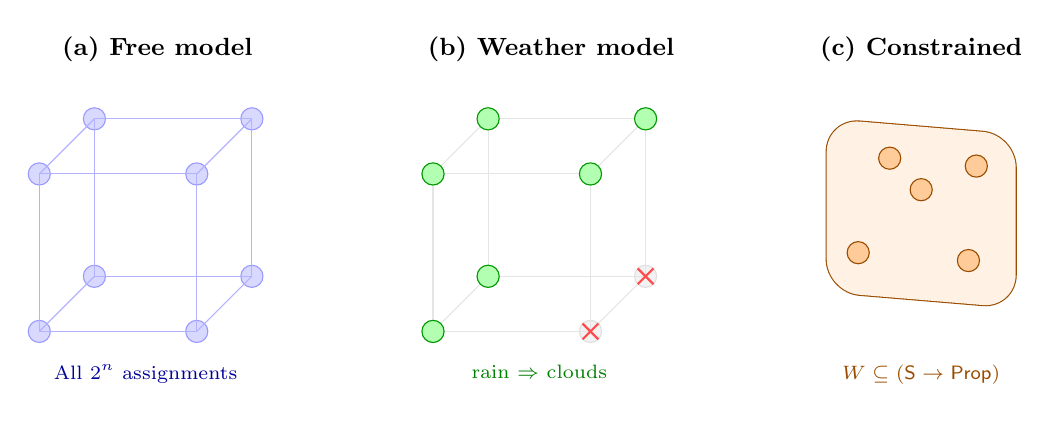
\begin{tikzpicture}[
  node distance=0.6cm,
  every node/.style={font=\small},
]
  % (a) Free model: full Boolean cube
  \begin{scope}[xshift=0cm]
    \node[font=\small\bfseries, anchor=south] at (1.5,3.3) {(a) Free model};
    % Draw a 3D cube of 8 vertices (all truth-value assignments)
    \foreach \x/\y in {0/0, 2/0, 0/2, 2/2} {
      \fill[blue!15, draw=blue!40] (\x,\y) circle (4pt);
    }
    \foreach \x/\y in {0.7/0.7, 2.7/0.7, 0.7/2.7, 2.7/2.7} {
      \fill[blue!15, draw=blue!40] (\x,\y) circle (4pt);
    }
    % Edges of cube
    \draw[blue!30, thin] (0,0)--(2,0)--(2,2)--(0,2)--cycle;
    \draw[blue!30, thin] (0.7,0.7)--(2.7,0.7)--(2.7,2.7)--(0.7,2.7)--cycle;
    \draw[blue!30, thin] (0,0)--(0.7,0.7) (2,0)--(2.7,0.7)
                          (0,2)--(0.7,2.7) (2,2)--(2.7,2.7);
    \node[font=\scriptsize, text=blue!60!black, anchor=north] at (1.35,-0.3)
      {All $2^n$ assignments};
  \end{scope}

  % (b) Weather model: shaded subset
  \begin{scope}[xshift=5.0cm]
    \node[font=\small\bfseries, anchor=south] at (1.5,3.3) {(b) Weather model};
    % Draw full cube ghosted
    \foreach \x/\y in {0/0, 2/0, 0/2, 2/2} {
      \fill[gray!10, draw=gray!25] (\x,\y) circle (4pt);
    }
    \foreach \x/\y in {0.7/0.7, 2.7/0.7, 0.7/2.7, 2.7/2.7} {
      \fill[gray!10, draw=gray!25] (\x,\y) circle (4pt);
    }
    \draw[gray!20, thin] (0,0)--(2,0)--(2,2)--(0,2)--cycle;
    \draw[gray!20, thin] (0.7,0.7)--(2.7,0.7)--(2.7,2.7)--(0.7,2.7)--cycle;
    \draw[gray!20, thin] (0,0)--(0.7,0.7) (2,0)--(2.7,0.7)
                          (0,2)--(0.7,2.7) (2,2)--(2.7,2.7);
    % Highlight valid worlds (rain->clouds satisfied)
    \foreach \x/\y in {0/0, 0/2, 2/2, 0.7/0.7, 0.7/2.7, 2.7/2.7} {
      \fill[green!30, draw=green!60!black] (\x,\y) circle (4pt);
    }
    % Cross out invalid worlds (rain=T, clouds=F)
    \foreach \x/\y in {2/0, 2.7/0.7} {
      \draw[red!70, thick] (\x-0.1,\y-0.1)--(\x+0.1,\y+0.1);
      \draw[red!70, thick] (\x-0.1,\y+0.1)--(\x+0.1,\y-0.1);
    }
    \node[font=\scriptsize, text=green!50!black, anchor=north] at (1.35,-0.3)
      {rain $\Rightarrow$ clouds};
  \end{scope}

  % (c) Abstract constrained model
  \begin{scope}[xshift=10.0cm]
    \node[font=\small\bfseries, anchor=south] at (1.2,3.3) {(c) Constrained};
    % Abstract blob
    \draw[orange!60!black, thick, rounded corners=12pt]
      (0,0.5) -- (2.4,0.3) -- (2.4,2.5) -- (0,2.7) -- cycle;
    \fill[orange!10, rounded corners=12pt]
      (0,0.5) -- (2.4,0.3) -- (2.4,2.5) -- (0,2.7) -- cycle;
    \foreach \x/\y in {0.4/1.0, 1.2/1.8, 1.8/0.9, 0.8/2.2, 1.9/2.1} {
      \fill[orange!40, draw=orange!60!black] (\x,\y) circle (4pt);
    }
    \node[font=\scriptsize, text=orange!60!black, anchor=north] at (1.2,-0.3)
      {$W \subseteq (\Sach \to \Prop)$};
  \end{scope}
\end{tikzpicture}
\caption{World-model architecture. (a)~The free model admits all
  $2^n$ truth-value assignments as worlds. (b)~The weather model
  excludes assignments violating rain $\Rightarrow$ clouds
  (crossed vertices). (c)~An abstract constrained model selects
  an arbitrary subset of the Boolean cube.  Compositionality
  holds in all three; independence holds only in~(a).}
\label{fig:worldmodels}
\end{figure}

% ================================================================
\section{Formal Limits: Expressibility and Equivalence}
\label{sec:limits}
% ================================================================

The deepest results of the formalization concern the boundaries
of what the object language can express.  These are not claims
within the Tractarian system but \emph{about} it---theorems at
the meta-level that formalize Wittgenstein's saying/showing
distinction.

% ----------------------------------------------------------------
\subsection{The \texttt{expresses} Relation}
\label{sec:expresses}
% ----------------------------------------------------------------

We introduce a typed bridge between the object language and the
metalanguage:

\begin{definition}[\texttt{expresses}]
\label{def:expresses}
A proposition $p : \mathsf{Proposition}\;\Sach$ \emph{expresses}
a meta-level property $P : \Prop$ if and only if $p$'s truth
value tracks $P$ in every world:
\[
  \expresses\;p\;P \;\;\stackrel{\mathrm{def}}{=}\;\;
  \forall\;w : \World\;\Sach,\;\; p.\eval\;w \leftrightarrow P
\]
\end{definition}

\begin{lstlisting}
def expresses (p : Proposition S) (P : Prop) : Prop :=
  ∀ w : World S, p.eval w ↔ P
\end{lstlisting}

\noindent
The type signature makes the object/meta distinction visible:
$p$ lives in the object language, $P$ lives in \Lean's
metalanguage, and \texttt{expresses} is the claim that they
correspond.  This is the formalization's key analytical device.

% ----------------------------------------------------------------
\subsection{Expressibility Collapse}
\label{sec:collapse}
% ----------------------------------------------------------------

\begin{theorem}[Expressibility collapse]
\label{thm:collapse}
If a proposition $p$ expresses a world-independent property
$P : \Prop$, then $p$ is a tautology or a contradiction.
\end{theorem}

\begin{proof}
Suppose $\expresses\;p\;P$ holds.  Then for any two worlds
$w_1, w_2$:
\[
  p.\eval\;w_1 \;\leftrightarrow\; P \;\leftrightarrow\;
  p.\eval\;w_2
\]
so $p$ has the same truth value in all worlds.  By excluded
middle on $p.\eval\;w_0$ for an arbitrary world~$w_0$, either
$p$ holds everywhere (tautology) or fails everywhere
(contradiction).
\end{proof}

\begin{lstlisting}
theorem saying_showing_triviality (q : Proposition S)
    (P : Prop)
    (h : expresses q P) :
    IsTautology q ∨ IsContradiction q := by
  apply world_constant_taut_or_contra
  intro w₁ w₂
  exact (h w₁).trans (h w₂).symm
\end{lstlisting}

\noindent
The contrapositive is immediate and philosophically sharper:

\begin{corollary}[Nontrivial propositions cannot express
world-independent content]
\label{cor:nontrivial}
If $p$ is nontrivial (i.e., true in some world and false in
another), then there is no $P : \Prop$ such that
$\expresses\;p\;P$.
\end{corollary}

\begin{lstlisting}
theorem nontrivial_cannot_express_world_independent
    (p : Proposition S) (P : Prop)
    (hnt : Nontrivial p) :
    ¬ expresses p P := by
  intro h
  exact nontrivial_expressibility_requires_world_dependence
    p P hnt h
\end{lstlisting}

\noindent
This is the paper's headline result.  It says: if a proposition
genuinely ``says'' something---i.e., carves out a nontrivial
region of logical space---then what it says cannot be a
world-independent truth.  Genuine content requires variation
across possible worlds.  What is world-independent can only be
``shown'' by the structure of the formalism itself, not ``said''
within it.

This transforms the saying/showing distinction from a
philosophical thesis into a provable constraint on
truth-functional languages.

\begin{remark}[On the definitional character of the collapse]
\label{rem:triviality}
A natural objection is that the expressibility collapse theorem
is \emph{trivial}: since $P : \Prop$ is world-independent by
construction (it is a closed term in \Lean's metalanguage), the
collapse to tautology or contradiction follows almost
definitionally from the definition of \texttt{expresses}.

We acknowledge this.  The proof is indeed short---two lines of
tactic code.  The contribution lies not in the proof's
difficulty but in three aspects of the \emph{formulation}:

\emph{(a) Making the object/meta boundary typed.}  The
definition of \texttt{expresses} forces the distinction between
$p : \mathsf{Proposition}\;\Sach$ (object language) and
$P : \Prop$ (metalanguage) to be a type-level constraint.  This
makes the boundary machine-checkable rather than merely
conventional.

\emph{(b) The analogy to other definitional results in logic.}
Many foundational results in logic are ``definitional'' in
a similar sense.  Tarski's undefinability theorem rests on the
diagonal lemma, which is itself a consequence of how truth
predicates are defined.  The incompleteness theorems depend on
the coding of syntax.  In each case, the contribution is the
\emph{conceptual apparatus} that makes the result statable, not
the complexity of the derivation.  Our \texttt{expresses}
relation plays an analogous role: it provides the vocabulary in
which the saying/showing distinction becomes a theorem.

\emph{(c) The constraint is genuinely informative.}
The collapse theorem rules out a precise class of claims:
no nontrivial proposition can serve as a ``name'' for a fixed
metalinguistic truth.  This is not obvious from the definition
of \texttt{expresses} alone---one must also establish
(via \texttt{world\_constant\_taut\_or\_contra}) that
world-invariant truth values force triviality.
\end{remark}

\begin{remark}[The \texttt{Nonempty S} assumption]
\label{rem:nonempty}
Exactly one theorem in the development requires
\texttt{[Nonempty S]} (i.e., that the type of states of affairs
is inhabited): \texttt{structEq\_ne\_semEq}, which must exhibit
a concrete elementary proposition and therefore needs at least
one atom.  (The separation witnesses of
Theorem~\ref{thm:hierarchy} take their two distinct atoms as
explicit hypotheses $a \neq b$ rather than assuming
inhabitation.)  The expressibility collapse
(Theorem~\ref{thm:collapse}) and its corollaries need no such
assumption: a witness world always exists, because
$\mathsf{World}\;\Sach = \Sach \to \Prop$ is inhabited by the
constant predicate $\lambda\,\_.\;\mathrm{True}$ even when
$\Sach$ is empty.  (For empty $\Sach$ the collapse is vacuous
for a different reason: $\mathsf{Proposition}\;\Sach$ has no
inhabitants, since every proposition bottoms out in an elementary
leaf.)  An earlier version of the formalization carried
\texttt{[Nonempty S]} on the collapse chain; removing it is a
small but genuine strengthening, and it locates the inhabitation
requirement exactly where it belongs: in the witnesses, which
must name atoms, not in the expressibility limits, which only
quantify over worlds.
\end{remark}

% ----------------------------------------------------------------
\subsection{What Can Be Said, Exactly}
\label{sec:whatcanbesaid}
% ----------------------------------------------------------------

The collapse theorem says what a proposition \emph{cannot}
express: a fixed world-independent truth $P : \Prop$.  Its
positive complement asks what a proposition \emph{can} express
when the meta-level content is allowed to depend on the world.
Say a property $P : \World\;\Sach \to \Prop$ is
\emph{invariant} if worlds agreeing pointwise up to $\iff$ agree
on $P$: for all $w_1, w_2$, if $\forall s.\; w_1\,s \iff w_2\,s$
then $P\,w_1 \iff P\,w_2$.  This is precisely the
truth-functional condition of
Section~\ref{sec:compositionality}, now imposed on a
metalinguistic predicate rather than derived for a proposition.
Over finitely many atoms, invariance is exactly expressibility
(\texttt{TractatusExpressibility.lean}):

\begin{theorem}[Exact characterization of the expressible]
\label{thm:expressible}
Let $\Sach$ be finite, decidable, and nonempty.  A world-property
$P : \World\;\Sach \to \Prop$ is expressible by some proposition
if and only if $P$ is invariant under pointwise-$\iff$ agreement
of worlds.
\end{theorem}

\begin{lstlisting}
theorem expressible_iff_iff_invariant {S : Type} [Fintype S]
    [DecidableEq S] [Nonempty S] (P : World S → Prop) :
    (∃ p : Proposition S, ∀ w : World S, p.eval w ↔ P w) ↔
    (∀ w₁ w₂ : World S, (∀ s, w₁ s ↔ w₂ s) → (P w₁ ↔ P w₂))
\end{lstlisting}

\noindent
The forward direction is truth-functional compositionality
(Theorem~\ref{thm:compositionality}): any property a proposition
expresses must respect pointwise-$\iff$ agreement, because the
proposition sees a world only through the truth-values of its
elementaries.  The backward direction is functional completeness
(Theorem~\ref{thm:fc}): an invariant $P$ descends to a Boolean
truth-function on assignments $\Sach \to \mathsf{Bool}$, which
some proposition realizes; \texttt{evalBool\_correct} transfers
the realization back to the $\Prop$-valued semantics.  The saying/
showing distinction thus has a sharp two-sided boundary over
finite atoms: the sayable is exactly the truth-functionally
invariant.

The finiteness hypothesis is not incidental.  A proposition has
only finitely many atoms, and its truth-value depends only on
them---a \emph{finite-support} property.  Let
$p.\mathtt{atoms}$ collect the elementaries occurring in $p$.

\begin{lemma}[Finite support]
\label{lem:finitesupport}
For any proposition $p$ and worlds $w_1, w_2$, if
$w_1\,s \iff w_2\,s$ for every $s \in p.\mathtt{atoms}$, then
$p.\mathtt{eval}\,w_1 \iff p.\mathtt{eval}\,w_2$.
\end{lemma}

\noindent
Over an infinite atom type, finite support defeats the very first
proposition of the \emph{Tractatus}.  TLP~1---``the world is
everything that is the case''---renders as the totality property
$\lambda w.\;\forall s.\; w\,s$.  This property \emph{is}
invariant under pointwise-$\iff$ agreement, so by
Theorem~\ref{thm:expressible} it would be expressible over any
finite $\Sach$.  Yet over an infinite $\Sach$ it is not:

\begin{theorem}[Inexpressibility of totality, TLP~1]
\label{thm:totality}
If $\Sach$ is infinite, no proposition expresses the totality
property: there is no $p$ with
$p.\mathtt{eval}\,w \iff (\forall s.\; w\,s)$ for all worlds~$w$.
\end{theorem}

\begin{lstlisting}
theorem totality_not_expressible {S : Type} [Infinite S] :
    ¬ ∃ p : Proposition S, ∀ w : World S, p.eval w ↔ (∀ s, w s)
\end{lstlisting}

\noindent
The proof compares the all-true world with the world true exactly
on $p.\mathtt{atoms}$.  The two agree on every atom of $p$, so by
finite support (Lemma~\ref{lem:finitesupport}) $p$ takes the same
value at both.  But totality holds at the first and---because an
infinite type has an atom outside the finite list
$p.\mathtt{atoms}$---fails at the second.  So no $p$ tracks
totality.  The three new results carry the same axiom footprint as
the rest of the Aristotle-assisted development
(\texttt{propext}, \texttt{Classical.choice},
\texttt{Quot.sound}).

\begin{remark}[The finite/infinite dichotomy]
\label{rem:dichotomy}
Theorems~\ref{thm:expressible} and~\ref{thm:totality} together
draw a sharp line.  For \emph{finitely} many atoms, invariance
and expressibility coincide: everything truth-functionally
invariant is sayable.  For \emph{infinitely} many atoms the two
come apart, and TLP~1 itself witnesses the gap---an invariant
property that no proposition expresses.

The reading this invites should be stated carefully, without
overclaiming.  The theorem is not a formal vindication of TLP~7 or
of the ladder metaphor (Section~\ref{sec:ladder}), and it does not
show that ``the world'' is unsayable \emph{simpliciter}.  It is a
result about \emph{this} object language over an infinite atom
type: within the finitary truth-functional syntax the
\emph{Tractatus} makes available, the totality of facts is not the
content of any proposition, even though it is a perfectly
well-defined predicate in the metalanguage that states the
theorem.  The unsayability is relative to the expressive means of
the object language, and it is the metalanguage---not silence---that
says it.  What the result does supply is a precise sense in which a
Tractarian language over infinitely many atoms cannot say, from
inside, that a given world is the whole of what is the case: the
gesture at totality lands outside the reach of the proposition.
\end{remark}

% ----------------------------------------------------------------
\subsection{Three Equivalence Relations}
\label{sec:hierarchy}
% ----------------------------------------------------------------

The formalization distinguishes three notions of proposition
equivalence:

\begin{definition}[Three equivalence relations]
\label{def:hierarchy}
Let $p, q : \mathsf{Proposition}\;\Sach$.
\begin{enumerate}[nosep]
  \item \textbf{Structural equivalence} ($p \structEq q$):
    $p$ and $q$ are built from identical constructors in the
    same tree shape with identical atoms.
  \item \textbf{Logical-form equivalence} ($p \formEq q$):
    there exists a bijective renaming of atoms (a permutation
    $\sigma : \Sach \xrightarrow{\sim} \Sach$) such that
    $p.\mathtt{rename}\;\sigma = q$.
  \item \textbf{Semantic equivalence} ($p \semEq q$):
    $p$ and $q$ have the same truth value in every world:
    $\forall w,\; p.\eval\;w \leftrightarrow q.\eval\;w$.
\end{enumerate}
\end{definition}

\noindent
We prove that $\formEq$ is an equivalence relation (reflexive by
the identity permutation, symmetric by inverse, transitive by
composition).  How do the three relations relate?  They do
\emph{not} form a chain.  Structural equivalence strictly refines
both coarser relations, but logical-form equivalence and semantic
equivalence are \emph{incomparable}: neither contains the other.

\begin{theorem}[Separation]
\label{thm:hierarchy}
As relations on $\mathsf{Proposition}\;\Sach$ (for $\Sach$ with
at least two atoms):
\begin{enumerate}[nosep]
  \item $\structEq \subsetneq \formEq$ and
        $\structEq \subsetneq \semEq$;
  \item $\formEq \not\subseteq \semEq$ and
        $\semEq \not\subseteq \formEq$;
  \item $\structEq \subsetneq \formEq \cap \semEq$.
\end{enumerate}
\end{theorem}

\begin{proof}
\emph{(1) Refinement.}  Structural equality implies propositional
equality (by induction), which implies logical-form equivalence
via the identity permutation
(\texttt{structEq\_implies\_formEq}) and semantic equivalence
trivially (\texttt{structEq\_implies\_semEq}).

\emph{(2) Incomparability.}
For any two distinct atoms $a \neq b$,
$\mathtt{elementary}(a)$ and $\mathtt{elementary}(b)$ are
$\formEq$ (via the swap permutation) but not $\semEq$: they
differ in truth value at the world where exactly~$a$ obtains
(\texttt{formEq\_not\_\allowbreak{}semEq\_\allowbreak{}witness}).  Conversely,
for any atom~$s$, $\lnot\lnot(\mathtt{elementary}\;s)$ is
$\semEq$ to $\mathtt{elementary}\;s$ (double negation) but not
$\formEq$, since renaming preserves tree depth
(\texttt{semEq\_not\_formEq\_witness}).  The same two pairs
witness strictness in~(1): the first separates $\structEq$ from
$\formEq$, the second separates $\structEq$ from $\semEq$.

\emph{(3) The intersection.}  For distinct atoms $a \neq b$,
the commuted conjunctions $a \wedge b$ and $b \wedge a$ share
their logical form (swap permutation) and their truth conditions
(commutativity of $\wedge$) yet are not structurally equal
(\texttt{formEq\_\allowbreak{}semEq\_\allowbreak{}not\_\allowbreak{}structEq\_\allowbreak{}witness}).  So even
the common refinement $\formEq \cap \semEq$ is strictly
coarser than $\structEq$.

All witnesses are stated in the formalization for an arbitrary
atom type~$\Sach$, taking the required distinct atoms as
explicit hypotheses; the running example
($\mathit{rain}$, $\mathit{snow}$ in \texttt{TwoFacts}) is
recovered as an instance, checked by \texttt{example}
declarations.  The theorem as stated is therefore machine-checked
at full generality.
\end{proof}

\begin{remark}[On truth-table isomorphism]
\label{rem:tt-iso}
What survives of the intuition that logical form is
``truth conditions up to relabeling''?  The formalization proves
\texttt{formEq\_implies\_truth\_table\_iso}: if
$p \formEq q$, there is a world-relabeling $f$ with
$p.\eval\;w \leftrightarrow q.\eval\;(f\;w)$ for all~$w$.
But this relation is far weaker than it looks, and the
formalization proves that too
(\texttt{truth\_table\_iso\_of\_\allowbreak{}nontrivial}): with
classical choice, \emph{any} proposition is
truth-table-isomorphic to \emph{any} nontrivial
proposition---relabel each world to a satisfying or refuting
world of~$q$ according to $p$'s truth value there.  So
truth-table isomorphism cannot serve as an intermediate notion
between $\formEq$ and $\semEq$; we record it as a lemma, not as
a rung of a hierarchy.
\end{remark}

% --- Equivalence Relations Figure ---
\begin{figure}[t]
\centering
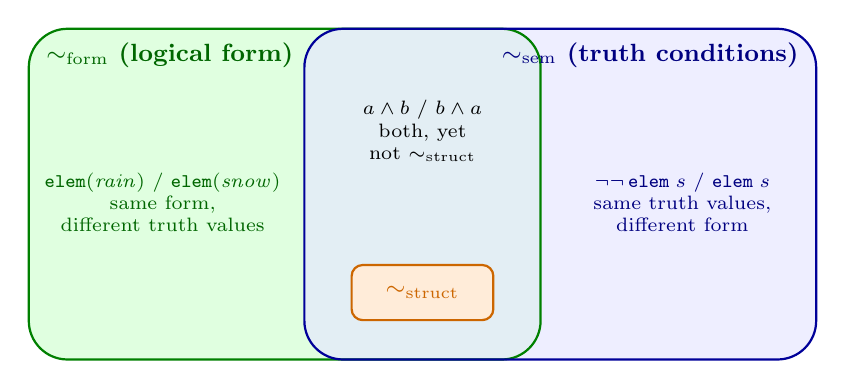
\begin{tikzpicture}[every node/.style={font=\small}]
  % Two overlapping regions: formEq (left) and semEq (right)
  \fill[green!12, rounded corners=14pt] (-5.0,-2.1) rectangle (1.5,2.1);
  \fill[blue!10, opacity=0.65, rounded corners=14pt] (-1.5,-2.1) rectangle (5.0,2.1);
  \draw[green!50!black, thick, rounded corners=14pt] (-5.0,-2.1) rectangle (1.5,2.1);
  \draw[blue!60!black, thick, rounded corners=14pt] (-1.5,-2.1) rectangle (5.0,2.1);

  % Region labels
  \node[font=\small\bfseries, text=green!40!black, anchor=north west]
    at (-4.9,2.05) {$\formEq$ (logical form)};
  \node[font=\small\bfseries, text=blue!50!black, anchor=north east]
    at (4.9,2.05) {$\semEq$ (truth conditions)};

  % structEq strictly inside the intersection
  \node[draw, thick, orange!80!black, fill=orange!15, rounded corners=4pt,
        minimum width=1.8cm, minimum height=0.7cm] at (0,-1.25) {$\structEq$};

  % Witnesses for each region
  \node[text=green!40!black, align=center, font=\scriptsize] at (-3.3,-0.1)
    {$\mathtt{elem}(\mathit{rain})$ / $\mathtt{elem}(\mathit{snow})$\\
     same form,\\ different truth values};
  \node[text=blue!50!black, align=center, font=\scriptsize] at (3.3,-0.1)
    {$\lnot\lnot\,\mathtt{elem}\;s$ / $\mathtt{elem}\;s$\\
     same truth values,\\ different form};
  \node[align=center, font=\scriptsize] at (0,0.8)
    {$a \wedge b$ / $b \wedge a$\\
     both, yet\\ not $\structEq$};
\end{tikzpicture}
\caption{The three equivalence relations.  $\formEq$ and $\semEq$
  are incomparable---each region contains a machine-checked
  witness---and $\structEq$ sits strictly inside their
  intersection (Theorem~\ref{thm:hierarchy}).}
\label{fig:hierarchy}
\end{figure}

\noindent
Figure~\ref{fig:hierarchy} illustrates the relationships.  This
clarifies a long-standing ambiguity in the
\emph{Tractatus}.  Wittgenstein's notion of ``logical form''
(TLP~4.0141) is neither syntactic identity nor truth-conditional
equivalence.  Our $\formEq$---defined via bijective atom
renaming---provides a formal candidate, and the separation
theorem shows it is genuinely independent of truth conditions:
form neither determines nor is determined by semantic content.
The two dimensions meet only above $\structEq$, and even their
intersection does not collapse to syntax
(part~3 of Theorem~\ref{thm:hierarchy}).

\begin{remark}[Relation to Tarskian invariance]
\label{rem:tarski}
Characterizing a notion by invariance under permutation recalls
Tarski's criterion of logicality~\cite{tarski1986}: a notion is
logical iff it is invariant under all permutations of the domain
of individuals.  Our $\formEq$ permutes \emph{atoms} to
characterize shared \emph{form between propositions}, rather
than permuting individuals to characterize \emph{logical
constants}; the two invariance criteria operate at different
levels.  The separation theorem adds something the Tarskian
tradition does not address: form-invariance and
truth-conditional identity cut across each other.  There is also
a structural echo of that tradition's central difficulty: just
as permutation invariance is charged with \emph{overgenerating}
logical constants~\cite{sher1991,bonnay2008}, our
\texttt{truth\_table\_iso\_of\_nontrivial}
(Remark~\ref{rem:tt-iso}) shows that world-relabeling
overgenerates equivalences---which is precisely why we do not
admit it as a rung between $\formEq$ and $\semEq$.
Spinney~\cite{spinney2022} gives a recent treatment of logical
form and logical space in the \emph{Tractatus} on which our
formal candidate can be brought to bear.
\end{remark}

% ----------------------------------------------------------------
\subsection{First-Order Extension}
\label{sec:firstorder}
% ----------------------------------------------------------------

In a companion file (\texttt{TractatusQuantifiers.lean}), we
extend the propositional calculus with first-order quantifiers
using higher-order abstract syntax (HOAS):

\begin{lstlisting}
inductive FOProp (S : Type) (D : Type) : Type where
  | lift     : Proposition S → FOProp S D
  | negFO    : FOProp S D → FOProp S D
  | conjFO   : FOProp S D → FOProp S D → FOProp S D
  | forall_  : (D → FOProp S D) → FOProp S D
  | exists_  : (D → FOProp S D) → FOProp S D
\end{lstlisting}

\noindent
The HOAS encoding leverages \Lean's metalanguage for variable
binding, avoiding explicit substitution machinery.  This
substantially reduces proof overhead but ties the formalization
more tightly to \Lean's metatheory than a de Bruijn index
encoding would---in particular, induction over HOAS terms
requires care, since the recursor for HOAS inductives must track
the functional argument.

We prove that compositionality lifts to the first-order level:

\begin{theorem}[First-order compositionality]
\label{thm:fo-comp}
For any $p : \mathsf{FOProp}\;\Sach\;D$ and worlds $w_1, w_2$
agreeing on all states of affairs, $p.\eval\;w_1 \leftrightarrow
p.\eval\;w_2$.
\end{theorem}

\noindent
We also establish eight additional results: universal--existential
duality (TLP~5.52), universal distribution over conjunction,
existential distribution over disjunction (reverse direction),
lift preservation, vacuous quantifier elimination (requiring
\texttt{Nonempty D}), double negation at the first-order level,
De Morgan duality for quantifiers, and first-order bivalence.

The results above are standard consequences of the semantic
definitions.  The philosophically loaded question is whether
Wittgenstein's $N$-operator can ground quantification
(TLP~5.52)---for infinite domains, Geach and
Soames~\cite{geach1981,soames1983} argue it cannot, since the
$N$-operator is a finitary syntactic operation.  We now settle
both directions of that question.

% ----------------------------------------------------------------
\subsection{The $N$-Operator: Finite Success, Infinite Failure}
\label{sec:noperator}
% ----------------------------------------------------------------

We formalize the $N$-operator as joint denial over a nonempty
argument list (TLP~5.502), in
\texttt{Tractatus\allowbreak{}NOperator\allowbreak{}.lean}:

\begin{lstlisting}
def NOp (p : Proposition S) (ps : List (Proposition S)) : Proposition S :=
  ps.foldl (fun acc q => Proposition.conj acc (Proposition.neg q))
    (Proposition.neg p)
\end{lstlisting}

\noindent
Its defining semantics is joint denial: $\mathtt{NOp}\;p\;ps$ is
true exactly when every argument is false (\texttt{NOp\_eval});
a first-order analogue \texttt{NOpFO} behaves identically.
Three consequences confirm TLP~5.5/5.512: binary $N$ is NOR,
unary $N$ is negation, and conjunction is $N(N(p), N(q))$---the
single operation suffices for the propositional basis.

For quantifiers, TLP~5.52 holds \emph{exactly} on finite
domains:

\begin{theorem}[TLP~5.52, finite domains]
\label{thm:tlp552}
Over a completely enumerated domain $d :: ds$ (every $x : D$
occurs in the list), for every family
$f : D \to \mathsf{FOProp}\;\Sach\;D$ and world $w$:
$\forall x.\,f x$ has the same truth value as
$N(\lnot f d, \lnot f d_1, \ldots)$, and $\exists x.\,f x$ the
same as $\lnot N(f d, f d_1, \ldots)$
(\texttt{forall\_as\_NOpFO}, \texttt{exists\_as\_NOpFO}).
\end{theorem}

\noindent
Conversely, the Geach--Soames critique is itself a theorem:

\begin{theorem}[Infinite-domain obstruction]
\label{thm:geach-soames}
Let $D$ be infinite and take atoms $\Sach = D$.  For every
choice of finitely many instances $d :: ds$, the $N$-application
$N(\lnot\,\mathtt{elementary}\;d, \lnot\,\mathtt{elementary}\;d_1,
\ldots)$ differs in truth value from
$\forall x.\,\mathtt{elementary}\;x$ at some world
(\texttt{no\_finite\_NOp\_for\_forall}).
\end{theorem}

\begin{proof}[Proof sketch]
Evaluate both sides at the world $w := (\cdot \in d :: ds)$.
The $N$-application is true there, since every listed instance
obtains; the universal quantifier is false, since an infinite
domain has an element outside any finite list.
\end{proof}

\noindent
This sharpens the dialectic of the expressive-completeness
debate: what Geach and Soames urged informally is, in this
reconstruction, a short countermodel.  What the theorem does
\emph{not} settle is Wittgenstein's own intent---whether
TLP~5.52's ``all values'' was ever meant as a finitary list.

\paragraph{Iterated $N$: TLP~6.}
The results above concern a \emph{single} $N$-application.
TLP~6 makes a stronger claim: every proposition arises from
the elementary propositions by \emph{successive} applications
of $N$.  We formalize the closure of the elementaries under
$N$ as an inductive predicate $\mathtt{NGen}$---the base case
is any elementary proposition, and the step case closes under
$\mathtt{NOp}\;p\;ps$ for $N$-generated $p$ and $ps$---and
prove that this closure exhausts the propositional fragment
up to semantic equivalence.

\begin{theorem}[$N$-generation completeness, TLP~6]
\label{thm:ngen}
For every proposition $p$ there is a proposition $q$ with
$\mathtt{NGen}\;q$ and $q \semEq p$: every proposition is
semantically equivalent to one built from elementary
propositions by iterated $N$-application
(\texttt{nGen\_complete}).
\end{theorem}

\begin{proof}[Proof sketch]
Induct on $p$.  An elementary proposition is $N$-generated
outright.  For $\lnot p$, take $N(q_p)$ where $q_p$ generates
$p$; unary $N$ is negation (\texttt{neg\_via\_NOp}), and
semantic equivalence is a congruence for $\lnot$
(\texttt{semEq\_neg\_congr}).  For $p \land r$, take
$N(N(q_p), N(q_r))$; this is conjunction
(\texttt{conj\_via\_NOp}), and semantic equivalence is a
congruence for $\land$ (\texttt{semEq\_conj\_congr}).
\end{proof}

\noindent
Combined with functional completeness
(Theorem~\ref{thm:fc}), the reach of iterated
joint denial is now exact: every truth-function over finitely
many atoms is realized by some proposition, and that
proposition is in turn semantically equivalent to one
generated from the elementaries by successive $N$.  This is
TLP~6's ``successive applications'' claim for the
propositional fragment, up to semantic equivalence.  What
remains open is the form-series \emph{notation}
$[\bar{p}, \bar{\xi}, N(\bar{\xi})]$ of TLP~6 itself and its
infinitary reading (see Section~\ref{sec:limitations}).

% ================================================================
\section{Related Work}
\label{sec:related}
% ================================================================

\paragraph{Formal reconstructions of the \emph{Tractatus}.}
Lokhorst~\cite{lokhorst1988} provides the most comprehensive
prior formal reconstruction, covering ontology, semantics, and
propositional attitudes in a set-theoretic framework.  His
axiomatization of independence and his truth-functionality
theorem (every sentence is a truth-function of elementary
sentences) overlap with our encoding, but he does not formalize
the saying/showing boundary itself.
Weiss~\cite{weiss2017} gives a 50-page reconstruction of the
\emph{Tractatus}'s logical system, analyzing the $N$-operator
and form-series in detail and proving that tautology-hood is
$\Pi^1_1$-complete for countable domains---a striking
complexity result that sharpens the Geach--Soames critique.
Miller~\cite{miller1995} develops a Tractarian semantics for
predicate logic that is independent of the metaphysics of
logical atomism, engaging with both Fogelin's~\cite{fogelin1987}
critique of expressive completeness and Carruthers'~\cite{carruthers1989}
book-length treatment of Tractarian semantics.
Stokhof~\cite{stokhof2008} reads the \emph{Tractatus} as a
proto-formal semantics, tracing its influence through Carnap's
state descriptions to possible-worlds semantics, and argues
that the saying/showing distinction arises from the
universalism of the framework---a philosophical diagnosis our
expressibility collapse theorem makes precise.
Spinney~\cite{spinney2022} examines the relation between logical
form and logical space in the \emph{Tractatus}; our
permutation-based $\formEq$ (Section~\ref{sec:hierarchy})
offers a formal candidate for the notion that discussion
targets.
All of these works provide formal clarity but are carried out
on paper; none offers machine-checked proofs, and none
parameterizes over world models to isolate which claims are
structural invariants versus modeling assumptions.

\paragraph{The expressive completeness debate.}
Fogelin~\cite{fogelin1987} initiates the modern debate over
whether the \emph{Tractatus}'s logical resources are
expressively complete.  Geach~\cite{geach1981} argues that the
$N$-operator cannot ground quantification over infinite domains,
since it is a finitary operation.
Soames~\cite{soames1983} sharpens this: the \emph{Tractatus}'s
claim that all of logic reduces to truth-functional operations
on elementary propositions is undermined when the domain of
quantification is infinite.
Carruthers~\cite{carruthers1989} provides a sympathetic
reconstruction of Tractarian semantics that attempts to address
some of these concerns.
Most recently, Lampert and Nakano~\cite{lampert2025} argue that
the classical undecidability proofs do not refute Wittgenstein's
early conception of logic on its own terms---he rejects
principles those proofs assume---and supply a purely logical
refutation that avoids such principles.  Our formalization is
neutral on this decidability dispute: we formalize the semantic
core (worlds, truth-functions, expressibility), not the
\emph{ab}-notation decision procedure whose fate that debate
concerns.
Our formalization engages the critique directly
(Section~\ref{sec:noperator}): TLP~5.52 is proved for finite
domains, and the infinite-domain failure is itself a
machine-checked theorem
(\texttt{no\_finite\_NOp\_for\_forall})---to our knowledge the
first formal rendering of the Geach--Soames objection.

\paragraph{Proof assistants and philosophy.}
Benzm\"uller and colleagues~\cite{benzmuller2017} have used
Isabelle to formalize ontological arguments and modal logic.
Their approach uses shallow semantic embeddings of higher-order
modal logic into Isabelle's metalogic, which contrasts with our
direct encoding in dependent type theory: we define the
Tractarian object language explicitly as an inductive type,
whereas shallow embeddings reuse the proof assistant's logic
as the object logic.
Fitelson and Zalta~\cite{fitelson2007} pioneer ``computational
metaphysics,'' using automated reasoners to verify theorems
in abstract-object theory.
Scherf~\cite{scherf2025} provides the most directly comparable
work: a machine-checked axiomatization of Advaita Ved\=anta in
\Lean~4 (69 axioms, 40+ theorems), demonstrating that complete
philosophical systems can be formalized in dependent type
theory.
Corfield~\cite{corfield2020} makes a sustained case for
homotopy type theory as a foundation for philosophical
reasoning, complementing the formal-verification approach
taken here.
To our knowledge, no prior work formalizes any part of the
\emph{Tractatus} in any proof assistant, nor uses the type
system to isolate the saying/showing boundary as a provable
constraint.

% ================================================================
\section{Discussion}
\label{sec:discussion}
% ================================================================

% ----------------------------------------------------------------
\subsection{What the Formalization Shows}
\label{sec:shows}
% ----------------------------------------------------------------

The formalization yields three kinds of insight.

First, it makes the \emph{Tractatus}'s implicit modeling
decisions explicit.  The choice $\World\;\Sach = \Sach \to
\Prop$ is not neutral: it builds independence into the
foundations.  By parameterizing over \texttt{WorldModel}, we
separate what follows from the propositional syntax (compositionality)
from what follows from the choice of world space (independence).
This distinction is available in principle but rarely made
precise in the philosophical literature.

Second, it transforms the saying/showing distinction from a
metaphilosophical thesis into a theorem with a two-line proof.
The \texttt{expresses} relation is the key: once the
object/meta boundary is a type distinction, the collapse result
(Theorem~\ref{thm:collapse}) follows by transitivity of
biconditional.  See Remark~\ref{rem:triviality} for a
discussion of the definitional character of this result and
why the formulation is nonetheless a genuine contribution.

Third, the separation theorem (Theorem~\ref{thm:hierarchy})
provides a precise formal candidate for Wittgenstein's
notion of ``logical form.''  The proved incomparability of
$\formEq$ and $\semEq$ shows that logical form, understood as
connective structure up to atom permutation, is not reducible to
truth conditions---and, conversely, that truth conditions do not
determine form.  The two are orthogonal dimensions of a
proposition's identity, meeting only above syntactic identity.

\begin{remark}[On automated proof search]
\label{rem:automation}
The $N$-operator and functional-completeness proofs were found
by an automated prover from our theorem statements (see the
Acknowledgments).  The division of labor is itself a datum for
this paper's theme: proof search automates what can be
\emph{said}---derivations of stated propositions---while the
choice of definitions (\texttt{expresses}, \texttt{formEq},
\texttt{NOp}, the world-model parameterization) is where the
philosophical content lives and resists delegation.
Statement-level errors are precisely the kind proof search
cannot catch: a prover asked to prove a false generalization
simply fails, while a reviewer can refute it.
\end{remark}

% ----------------------------------------------------------------
\subsection{Limitations}
\label{sec:limitations}
% ----------------------------------------------------------------

Several aspects of the \emph{Tractatus} lie beyond the scope of
this formalization.

\paragraph{Object structure.}
The type $\Sach$ is abstract: we do not model how objects combine
into states of affairs.  TLP~2.0141 (``The possibility of its
occurrence in atomic facts is the form of the object'') suggests
a richer dependent-type encoding where the form of an object
constrains its combinatorial possibilities.  This would make
independence a substantive theorem rather than a definitional
consequence.

\paragraph{The form-series.}
The $N$-operator is formalized
(Section~\ref{sec:noperator}), and Wittgenstein's claim that
all propositions arise by \emph{successive} applications of
$N$ now holds for the propositional fragment up to semantic
equivalence: every proposition is semantically equivalent to
one generated from the elementaries by iterated $N$
(Theorem~\ref{thm:ngen}).  What remains open is the
form-series \emph{notation} of TLP~6 itself,
$[\bar{p}, \bar{\xi}, N(\bar{\xi})]$, together with its
infinitary reading---the recursive schema in which the same
operation is applied to its own results without bound.  Our
$\mathtt{NGen}$ closure is finitary and unstructured (a mere
inductive predicate), not Wittgenstein's indexed general form
of the proposition.

\paragraph{The picture theory.}
The \emph{Tractatus}'s claim that propositions are
\emph{pictures} of reality (TLP~2.1--2.174) involves a notion
of structural isomorphism between language and world that goes
beyond truth-functional evaluation.  Our formalization captures
the truth-conditional aspect but not the pictorial-isomorphism
aspect.

\paragraph{Self-reference and the ladder.}
\label{sec:ladder}
TLP~6.54 famously declares that the propositions of the
\emph{Tractatus} itself are ``nonsensical'' and must be ``thrown
away'' after use.  Our formalization is, by design, a
metalanguage that talks \emph{about} the Tractarian object
language.  It cannot formalize its own status as a ladder to be
discarded---this is the point where type theory, like any formal
system, reaches its own saying/showing boundary.

We mark this boundary with a deliberate axiom:

\begin{lstlisting}
axiom silence : True
\end{lstlisting}

\noindent
This is not a missing proof but a design boundary.  The axiom
states nothing contentful ($\mathtt{True}$ is already provable);
it marks the point where the formalization acknowledges its own
limits.

\begin{remark}[Why \texttt{True}]
\label{rem:why-true}
The choice of \texttt{True} as the axiom's type is deliberate.
Because \texttt{True} is already provable in \Lean{} (via
\texttt{trivial}), the axiom \texttt{silence} adds no logical
content whatsoever---it introduces no new assumptions and
changes no proof obligations.  Its content is its \emph{label},
not its type.  The name ``silence'' marks a boundary; the
type \texttt{True} ensures that boundary is inert.  This
mirrors TLP~7's status as a proposition that, by Wittgenstein's
own account, says nothing: it is a gesture toward what lies
beyond the expressible, not an assertion within it.
\end{remark}

% ----------------------------------------------------------------
\subsection{Beyond the Tractatus}
\label{sec:beyond}
% ----------------------------------------------------------------

The expressibility collapse theorem
(Theorem~\ref{thm:collapse}) is formulated in terms of
Tractarian propositions, but it depends only on two structural
features: (i)~the object language is truth-functional
(proposition truth values are determined by evaluation against
worlds), and (ii)~the metalanguage is typed, so that a
``world-independent property'' is simply a term of type
$\Prop$ with no free world variable.  Any truth-functional
object language embedded in a typed metalanguage with this
structure will exhibit the same collapse.

This means the result is not specific to the
\emph{Tractatus}.  Classical propositional logic, Boolean
algebras interpreted over sets of valuations, and modal
propositional logics (when the accessibility relation is
removed) all satisfy the preconditions.  The collapse theorem
is a general fact about the typed embedding of truth-functional
languages: the type system enforces a gap between
world-dependent content (nontrivial propositions) and
world-independent truth (metalinguistic facts), and no
nontrivial proposition can bridge it.

For logicians who may not share an interest in Wittgenstein
exegesis, this generality is the main takeaway: the
saying/showing distinction, stripped of its philosophical
mystique, is a typing constraint that any truth-functional
formalization must respect.

% ----------------------------------------------------------------
\subsection{Future Work}
\label{sec:future}
% ----------------------------------------------------------------

Several directions for further investigation arise naturally.
First, with iterated $N$-application now settled up to
semantic equivalence (Theorem~\ref{thm:ngen}), the remaining
form-series work is to formalize TLP~6's general propositional
form $[\bar{p}, \bar{\xi}, N(\bar{\xi})]$ as an indexed
recursive schema---and to give its infinitary reading a
coherent semantics---rather than the finitary, unstructured
$\mathtt{NGen}$ closure we prove complete here.
Second, encoding object structure via dependent types---so
that states of affairs are typed combinations of objects
constrained by form (TLP~2.0141)---would make independence
a substantive theorem rather than a definitional consequence
of the world type.
Third, extending the \texttt{expresses} relation to
world-dependent properties ($P : \World\;\Sach \to \Prop$)
would allow a finer analysis of what nontrivial propositions
\emph{can} express, complementing the current result about
what they cannot.
Fourth, formalizing the doxastic extension of Tractarian
semantics along the lines of Lokhorst~\cite{lokhorst1988}
would test whether the invariant/assumption/limit decomposition
extends to propositional attitudes.
Fifth, a companion development by the author already generalizes
the constrained countermodels of Section~\ref{sec:assumptions}
to arbitrary lists of Horn-clause constraints (and biconditional
constraints via symmetric closure), and organizes world models
under a refinement preorder with the free model as maximum;
integrating that material would deepen the assumption tier of
the decomposition.

% ================================================================
\section{Conclusion}
\label{sec:conclusion}
% ================================================================

We have presented a machine-checked reconstruction of the
semantic core of \emph{Tractatus Logico-Philosophicus} in
\Lean~4.  The formalization proves 77 formally verified results
across five files, decomposes the
\emph{Tractatus} into structural invariants, model-dependent
assumptions, and formal limits of expressibility, and
characterizes the saying/showing distinction as a theorem:
nontrivial propositions cannot express world-independent truths.
It settles TLP~5.52 in both directions---the $N$-operator grounds
quantification over finite domains and provably fails to over
infinite ones---and proves TLP~5.101 in full strength.
It also fixes the sayable exactly: over finitely many atoms a
world-property is expressible iff it is invariant under
pointwise-$\iff$ agreement of worlds, while over infinitely many
atoms the totality property of TLP~1 is invariant yet expressed by
no proposition---so the totality of facts, sayable in the
metalanguage, lies outside the reach of the object language whose
propositions have finite support.

The equivalence analysis separates three relations on
propositions: syntactic identity strictly refines logical-form
equivalence and semantic equivalence, which are themselves
provably incomparable.  Logical form is thus not a way-station
between syntax and truth conditions but an independent dimension
of a proposition's identity---a reading of TLP~4.0141 that only
becomes visible under formalization.

These results suggest that proof assistants are a productive tool
for philosophical analysis---not merely for verifying known
results, but for revealing structural constraints that are
invisible when the analysis is conducted on paper.

The formalization is publicly available at
\url{https://github.com/rjwalters/tractatus}, with a
browsable proof gallery at
\url{https://leangenius.org/proof/tractatus-ontology}.

\section*{Acknowledgments}

The proofs in \texttt{TractatusNOperator.lean},
\texttt{TractatusCompleteness.lean}, and
\texttt{TractatusExpressibility.lean} were produced by Harmonic's
Aristotle automated theorem prover~\cite{harmonic2026} from
theorem statements authored by us (submitted with \texttt{sorry}
placeholders; statements unchanged), and were re-verified by the
\Lean{} kernel against the repository's pinned toolchain.  Their
axiom footprint is \texttt{propext}, \texttt{Classical.choice},
\texttt{Quot.sound} only.  For
\texttt{TractatusExpressibility.lean}, the support the Aristotle
problem files inlined (re-declared syntax and semantics, the
Bool-valued evaluator, truth-functional compositionality, and the
disjunctive-normal-form construction) is de-duplicated against the
built development; only the three headline
statements---\texttt{expressible\_iff\_iff\_invariant},
\texttt{eval\_depends\_only\_on\_atoms}, and
\texttt{totality\_not\_expressible}---and their finite-support
scaffolding remain.  All definitions, theorem statements, and the
remaining proofs are ours.

% ================================================================
% Appendix
% ================================================================

\appendix

% ----------------------------------------------------------------
\section{Build Instructions}
\label{app:build}
% ----------------------------------------------------------------

The formalization is built with \Lean~4 using the \texttt{lake}
build system.  To reproduce:

\begin{enumerate}[nosep]
  \item Install \Lean~4 via \texttt{elan}:\\
    {\small\ttfamily curl -sSf https://raw.githubusercontent.com/\allowbreak{}leanprover/\allowbreak{}elan/\allowbreak{}master/\allowbreak{}elan-init.sh | sh}
  \item Clone the repository:\\
    {\small\ttfamily git clone https://github.com/rjwalters/tractatus.git}
  \item The \texttt{lean-toolchain} file pins the version to
    {\small\ttfamily leanprover/lean4:v4.26.0}.
  \item The \texttt{lakefile.lean} declares a dependency on
    Mathlib (the formalization uses
    {\small\ttfamily import Mathlib.Tactic}).
  \item Build: {\small\ttfamily lake build}
\end{enumerate}

\noindent
The build produces zero errors, zero warnings, and zero
\texttt{sorry} obligations.  A GitHub Actions workflow in the
repository runs \texttt{lake build} on every push, so the build
status of the public sources is continuously verified.  The sole axiom
(\texttt{axiom silence : True}) is intentional and
discussed in Section~\ref{sec:limitations}.

Proof files:
\begin{itemize}[nosep]
  \item \texttt{proofs/TractatusOntology.lean} --- 1,345 lines, 45 declarations
  \item \texttt{proofs/TractatusQuantifiers.lean} --- 284 lines, 9 declarations
  \item \texttt{proofs/TractatusNOperator.lean} --- 239 lines, 11 declarations
  \item \texttt{proofs/TractatusCompleteness.lean} --- 142 lines, 9 declarations
  \item \texttt{proofs/TractatusExpressibility.lean} --- 138 lines, 3 declarations
\end{itemize}

% ----------------------------------------------------------------
\section{Complete Theorem Listing}
\label{app:theorems}
% ----------------------------------------------------------------

Table~\ref{tab:decomposition} classifies every theorem and lemma
declaration in the formalization.  The ``Class'' column indicates
whether the result is a structural \textbf{I}nvariant,
a model-dependent \textbf{A}ssumption or counterexample, or a
formal \textbf{L}imit on expressibility.  Results marked
\textbf{H} are helper lemmas for the equivalence apparatus
(renaming and \texttt{formEq}).
Results marked \textbf{E} are engineering artifacts
(Bool-valued evaluation).  All Lean names are given in full;
they can be located in the source files by exact text search.

\begin{table}[p]
\centering
\footnotesize
\caption{Complete listing of all 77 theorem/lemma declarations
  plus 1 axiom, classified by the three-way decomposition.
  \textbf{I}~=~invariant, \textbf{A}~=~assumption/counterexample,
  \textbf{L}~=~limit, \textbf{H}~=~equivalence helper,
  \textbf{E}~=~engineering.}
\label{tab:decomposition}
\begin{tabular}{@{}rlllc@{}}
\toprule
\# & \textbf{Lean name} & \textbf{TLP} & \textbf{File} & \textbf{Cl.} \\
\midrule
\multicolumn{5}{l}{\emph{TractatusOntology.lean} (45 declarations)} \\
\midrule
 1 & \texttt{evalBool\_correct}                        & 5.1     & Ont. & E \\
 2 & \texttt{truth\_functional\_compositionality\_gen}  & 5       & Ont. & I \\
 3 & \texttt{evalM\_free\_eq\_eval}                     & ---     & Ont. & I \\
 4 & \texttt{tautology\_is\_world\_invariant}            & 6.1     & Ont. & I \\
 5 & \texttt{contradiction\_holds\_nowhere}              & 4.46    & Ont. & I \\
 6 & \texttt{elem\_prop\_bivalence}                      & 4.023   & Ont. & I \\
 7 & \texttt{truth\_functional\_compositionality}        & 5       & Ont. & I \\
 8 & \texttt{elementary\_independence}                   & 2.061   & Ont. & A \\
 9 & \texttt{double\_negation}                           & 5.101   & Ont. & I \\
10 & \texttt{de\_morgan\_disj}                           & 5.101   & Ont. & I \\
11 & \texttt{de\_morgan\_conj}                           & 5.101   & Ont. & I \\
12 & \texttt{excluded\_middle\_tautology}                & 4.46    & Ont. & I \\
13 & \texttt{conj\_neg\_contradiction}                   & 4.46    & Ont. & I \\
14 & \texttt{impl\_semantics}                            & 5.101   & Ont. & I \\
15 & \texttt{biimp\_semantics}                           & 5.101   & Ont. & I \\
16 & \texttt{modus\_ponens}                              & 4.121   & Ont. & I \\
17 & \texttt{nand\_expresses\_neg}                       & 5.5     & Ont. & I \\
18 & \texttt{nand\_expresses\_conj}                      & 5.5     & Ont. & I \\
19 & \texttt{constrained\_independence\_fails}           & 2.061   & Ont. & A \\
20 & \texttt{weather\_independence\_fails}               & 2.061   & Ont. & A \\
21 & \texttt{rename\_id}                                 & 4.014   & Ont. & H \\
22 & \texttt{rename\_comp}                               & 4.014   & Ont. & H \\
23 & \texttt{rename\_eval}                               & 4.014   & Ont. & H \\
24 & \texttt{formEq\_refl}                               & 4.0141  & Ont. & H \\
25 & \texttt{formEq\_symm}                               & 4.0141  & Ont. & H \\
26 & \texttt{formEq\_trans}                              & 4.0141  & Ont. & H \\
27 & \texttt{eq\_of\_structEq} (private)                 & 4.0141  & Ont. & H \\
28 & \texttt{structEq\_implies\_formEq}                  & 4.0141  & Ont. & L \\
29 & \texttt{structEq\_implies\_semEq}                   & 4.0141  & Ont. & L \\
30 & \texttt{formEq\_implies\_truth\_table\_iso}         & 4.0141  & Ont. & L \\
31 & \texttt{truth\_table\_iso\_id\_implies\_semEq}      & 4.0141  & Ont. & L \\
32 & \texttt{truth\_table\_iso\_of\_nontrivial}          & 4.0141  & Ont. & L \\
33 & \texttt{formEq\_not\_structEq\_witness}             & 4.0141  & Ont. & L \\
34 & \texttt{semEq\_not\_formEq\_witness}                & 4.0141  & Ont. & L \\
35 & \texttt{formEq\_not\_semEq\_witness}                & 4.0141  & Ont. & L \\
36 & \texttt{formEq\_semEq\_not\_structEq\_witness}      & 4.0141  & Ont. & L \\
37 & \texttt{structEq\_ne\_semEq}                        & 4.0141  & Ont. & L \\
38 & \texttt{world\_constant\_taut\_or\_contra}          & 4.46    & Ont. & L \\
39 & \texttt{saying\_showing\_triviality}                & 4.12    & Ont. & L \\
40 & \texttt{contingent\_propositions\_vary}             & 4.46    & Ont. & L \\
41 & \texttt{nontrivial\_of\_not\_taut\_not\_contra}     & 4.46    & Ont. & L \\
42 & \texttt{nontrivial\_iff\_not\_taut\_not\_contra}    & 4.46    & Ont. & L \\
43 & \texttt{proposition\_seven}                         & 7       & Ont. & L \\
44 & \texttt{nontrivial\_expressibility\_requires\_world\_dependence}
                                                         & 4.12    & Ont. & L \\
45 & \texttt{nontrivial\_cannot\_express\_world\_independent}
                                                         & 4.12    & Ont. & L \\
\midrule
\multicolumn{5}{l}{\emph{TractatusQuantifiers.lean} (9 declarations)} \\
\midrule
46 & \texttt{truth\_functional\_compositionality\_fo}    & 5       & Quant. & I \\
47 & \texttt{forall\_exists\_duality}                    & 5.52    & Quant. & I \\
48 & \texttt{forall\_distrib\_conj}                      & 5.52    & Quant. & I \\
49 & \texttt{exists\_distrib\_disj\_reverse}             & 5.52    & Quant. & I \\
50 & \texttt{lift\_eval}                                 & ---     & Quant. & I \\
51 & \texttt{forall\_vacuous}                            & ---     & Quant. & I \\
52 & \texttt{double\_negation\_fo}                       & 5.101   & Quant. & I \\
53 & \texttt{not\_exists\_forall\_not}                   & 5.52    & Quant. & I \\
54 & \texttt{fo\_bivalence}                              & 4.023   & Quant. & I \\
\midrule
\multicolumn{5}{l}{\emph{TractatusNOperator.lean} (11 declarations)} \\
\midrule
55 & \texttt{NOp\_eval}                                 & 5.502   & NOp. & I \\
56 & \texttt{NOpFO\_eval}                               & 5.502   & NOp. & I \\
57 & \texttt{NOp\_pair\_eval}                           & 5.5     & NOp. & I \\
58 & \texttt{neg\_via\_NOp}                             & 5.512   & NOp. & I \\
59 & \texttt{conj\_via\_NOp}                            & 5.5     & NOp. & I \\
60 & \texttt{forall\_as\_NOpFO}                         & 5.52    & NOp. & I \\
61 & \texttt{exists\_as\_NOpFO}                         & 5.52    & NOp. & I \\
62 & \texttt{no\_finite\_NOp\_for\_forall}              & 5.52    & NOp. & L \\
63 & \texttt{semEq\_neg\_congr}                         & 6       & NOp. & H \\
64 & \texttt{semEq\_conj\_congr}                        & 6       & NOp. & H \\
65 & \texttt{nGen\_complete}                            & 6       & NOp. & I \\
\midrule
\multicolumn{5}{l}{\emph{TractatusCompleteness.lean} (9 declarations)} \\
\midrule
66 & \texttt{disj\_evalBool}                            & 5.101   & Comp. & E \\
67 & \texttt{literal\_evalBool}                         & 5.101   & Comp. & E \\
68 & \texttt{truePropOf\_evalBool}                      & 5.101   & Comp. & E \\
69 & \texttt{falsePropOf\_evalBool}                     & 5.101   & Comp. & E \\
70 & \texttt{conjFold\_evalBool}                        & 5.101   & Comp. & E \\
71 & \texttt{minterm\_evalBool}                         & 5.101   & Comp. & E \\
72 & \texttt{bigDisj\_evalBool}                         & 5.101   & Comp. & E \\
73 & \texttt{dnf\_evalBool}                             & 5.101   & Comp. & E \\
74 & \texttt{functional\_completeness}                  & 5.101   & Comp. & I \\
\midrule
\multicolumn{5}{l}{\emph{TractatusExpressibility.lean} (3 declarations)} \\
\midrule
75 & \texttt{expressible\_iff\_iff\_invariant}          & 5       & Expr. & L \\
76 & \texttt{eval\_depends\_only\_on\_atoms}            & 5       & Expr. & L \\
77 & \texttt{totality\_not\_expressible}                & 1       & Expr. & L \\
\midrule
\multicolumn{5}{l}{\emph{Axiom}} \\
\midrule
--- & \texttt{axiom silence : True}                      & 7       & Ont. & L \\
\bottomrule
\end{tabular}
\end{table}

% ================================================================
% References
% ================================================================

\begin{thebibliography}{99}

\bibitem{wittgenstein1921}
L.~Wittgenstein,
\emph{Tractatus Logico-Philosophicus},
Kegan Paul, 1921.
Translated by C.~K. Ogden; reprinted by Routledge, 2001.

\bibitem{wittgenstein1929}
L.~Wittgenstein,
``Some remarks on logical form,''
\emph{Proceedings of the Aristotelian Society, Supplementary
Volumes}, vol.~9, pp.~162--171, 1929.

\bibitem{lokhorst1988}
G.-J.~C. Lokhorst,
``Ontology, semantics and philosophy of mind in Wittgenstein's
\emph{Tractatus}: A formal reconstruction,''
\emph{Erkenntnis}, vol.~29, no.~1, pp.~35--75, 1988.
\newline doi:~\href{https://doi.org/10.1007/BF00166365}{\texttt{10.1007/BF00166365}}.

\bibitem{fogelin1987}
R.~J. Fogelin,
\emph{Wittgenstein}, 2nd ed.,
London: Routledge, 1987.
(First edition 1976.)

\bibitem{carruthers1989}
P.~Carruthers,
\emph{Tractarian Semantics: Finding Sense in Wittgenstein's
\emph{Tractatus}},
Oxford: Blackwell, 1989.

\bibitem{stokhof2008}
M.~Stokhof,
``The architecture of meaning: Wittgenstein's \emph{Tractatus} and
formal semantics,''
in \emph{Wittgenstein's Enduring Arguments},
D.~Levy and E.~Zamuner, Eds.\
London: Routledge, 2008, pp.~211--244.

\bibitem{weiss2017}
M.~Weiss,
``Logic in the \emph{Tractatus},''
\emph{The Review of Symbolic Logic}, vol.~10, no.~1,
pp.~1--50, 2017.
\newline doi:~\href{https://doi.org/10.1017/S1755020316000472}{\texttt{10.1017/S1755020316000472}}.

\bibitem{geach1981}
P.~T.~Geach,
``Wittgenstein's operator $N$,''
\emph{Analysis}, vol.~41, no.~4, pp.~168--171, 1981.
\newline doi:~\href{https://doi.org/10.1093/analys/41.4.168}{\texttt{10.1093/analys/41.4.168}}.

\bibitem{soames1983}
S.~Soames,
``Generality, truth functions, and expressive capacity in the
\emph{Tractatus},''
\emph{The Philosophical Review}, vol.~92, no.~4, pp.~573--589, 1983.
\newline doi:~\href{https://doi.org/10.2307/2184881}{\texttt{10.2307/2184881}}.

\bibitem{miller1995}
H.~Miller,
``Tractarian semantics for predicate logic,''
\emph{History and Philosophy of Logic}, vol.~16, no.~2,
pp.~197--215, 1995.
\newline doi:~\href{https://doi.org/10.1080/01445349508837249}{\texttt{10.1080/01445349508837249}}.

\bibitem{benzmuller2017}
C.~Benzm\"uller and B.~Woltzenlogel Paleo,
``An object-logic explanation of the inconsistency in G\"odel's
ontological theory,''
\emph{Journal of Applied Logic}, vol.~24, pp.~253--265, 2017.
\newline doi:~\href{https://doi.org/10.1016/j.jal.2017.01.001}{\texttt{10.1016/j.jal.2017.01.001}}.

\bibitem{fitelson2007}
B.~Fitelson and E.~N. Zalta,
``Steps toward a computational metaphysics,''
\emph{Journal of Philosophical Logic}, vol.~36, no.~2,
pp.~227--247, 2007.
\newline doi:~\href{https://doi.org/10.1007/s10992-006-9038-7}{\texttt{10.1007/s10992-006-9038-7}}.

\bibitem{scherf2025}
M.~Scherf,
``The formal logic of Advaita Ved\=anta: A complete
axiomatization and consistency proof,''
Unpublished manuscript, 2025.
Original repository \texttt{github.com/matthew-scherf/Advaita}
(since removed); archived at
\url{https://web.archive.org/web/20260219072022/https://github.com/matthew-scherf/advaita}.

\bibitem{harmonic2026}
Harmonic,
\emph{Aristotle} (automated theorem prover for \Lean~4), 2026.
Available: \url{https://aristotle.harmonic.fun}.
Accessed 2026-07-12.

\bibitem{lampert2025}
T.~Lampert and A.~Nakano,
``A logical refutation of Wittgenstein's early philosophy of
logic,''
\emph{History and Philosophy of Logic}, pp.~1--19, 2025.
\newline doi:~\href{https://doi.org/10.1080/01445340.2025.2498308}{\texttt{10.1080/01445340.2025.2498308}}.

\bibitem{sher1991}
G.~Sher,
\emph{The Bounds of Logic: A Generalized Viewpoint},
MIT Press, 1991.

\bibitem{bonnay2008}
D.~Bonnay,
``Logicality and invariance,''
\emph{Bulletin of Symbolic Logic}, vol.~14, no.~1, pp.~29--68,
2008.
\newline doi:~\href{https://doi.org/10.2178/bsl/1208358843}{\texttt{10.2178/bsl/1208358843}}.

\bibitem{tarski1986}
A.~Tarski,
``What are logical notions?''
(ed.\ J.~Corcoran),
\emph{History and Philosophy of Logic}, vol.~7, no.~2,
pp.~143--154, 1986.
\newline doi:~\href{https://doi.org/10.1080/01445348608837096}{\texttt{10.1080/01445348608837096}}.

\bibitem{spinney2022}
O.~T.~Spinney,
``Logical form and logical space in Wittgenstein's
\emph{Tractatus},''
\emph{Synthese}, vol.~200, article~16, 2022.
\newline doi:~\href{https://doi.org/10.1007/s11229-022-03470-y}{\texttt{10.1007/s11229-022-03470-y}}.

\bibitem{corfield2020}
D.~Corfield,
\emph{Modal Homotopy Type Theory: The Prospect of a New Logic
for Philosophy},
Oxford University Press, 2020.
\newline doi:~\href{https://doi.org/10.1093/oso/9780198853404.001.0001}{\texttt{10.1093/oso/9780198853404.001.0001}}.

\bibitem{moura2021}
L.~de Moura and S.~Ullrich,
``The \textsc{Lean}~4 theorem prover and programming language,''
in \emph{Proceedings of CADE-28}, Springer LNCS, 2021.
\newline doi:~\href{https://doi.org/10.1007/978-3-030-79876-5_37}{\texttt{10.1007/978-3-030-79876-5\_37}}.

\end{thebibliography}

\end{document}
